\documentclass[]{article}
\usepackage{amsmath}
\usepackage{amsthm}
\usepackage{listings}
\usepackage{graphicx}

\title{Practical Lab Numerical Computing Computational Finance \\Bachelor-Worksheet 3}
\author{Lukas Troska, Ilja Kalmykov}
\date{}
\setlength{\parindent}{0pt}

\begin{document}

\maketitle
\section*{Task 2}
See task2.cpp for code.

\section*{Task 3}
As we can see, the number of timesteps does not affect the convergence at all.\\
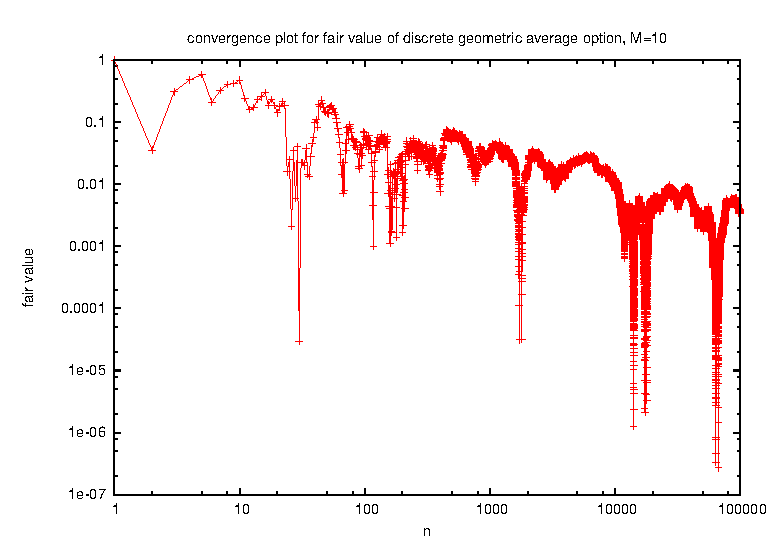
\includegraphics{task3_10.eps}\\
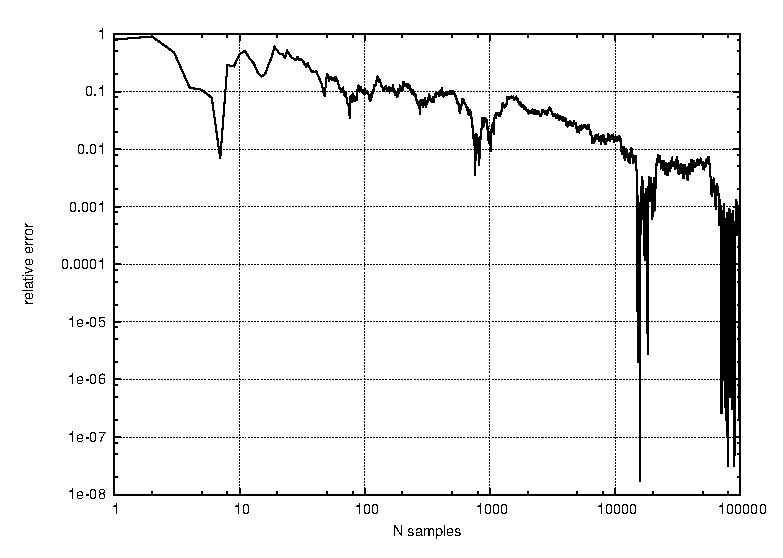
\includegraphics{task3_200.eps}\\

\section*{Task 4}
See task4.cpp for code. The convergence is $N^{-0.5}$(????). The last increase in error is because of the limitations of the datatype int. For $M\ge 1024$ we get under-/overflows in our calculation because the numbers are too big.
\\
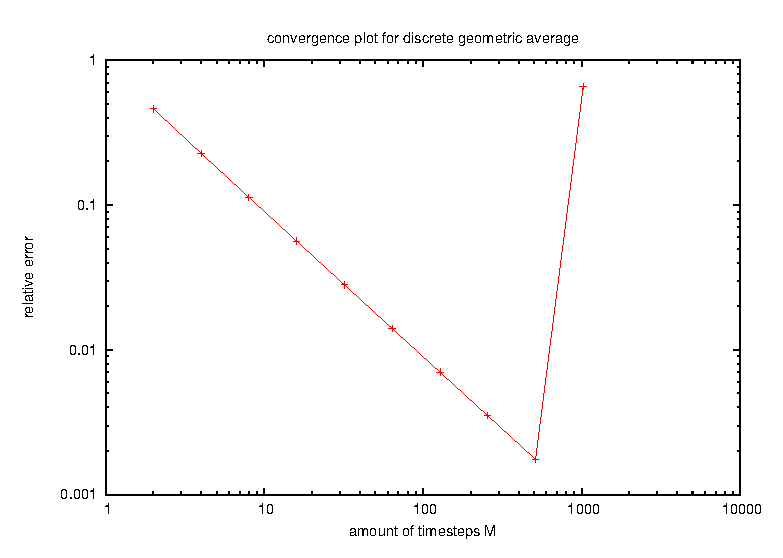
\includegraphics{task4.eps}\\

\section*{Task 5}
See task5.cpp for code. The integrand of the discrete arithmetic average for $M=2$ looks like:\\
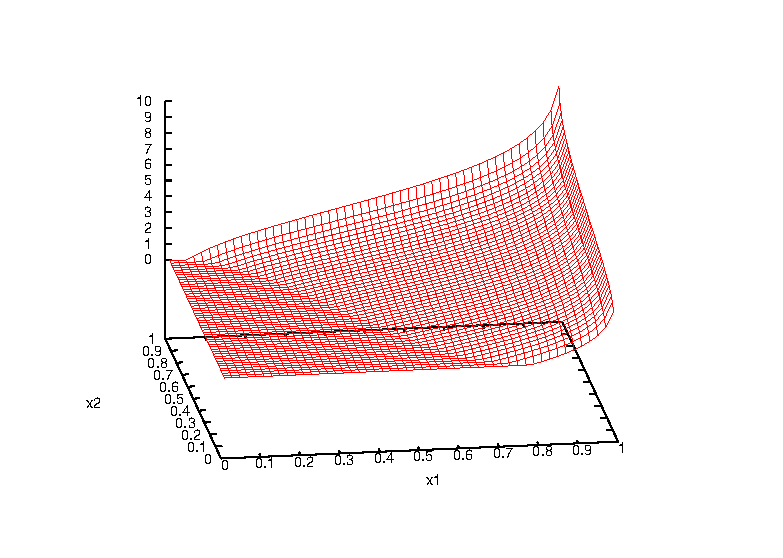
\includegraphics{task5_1}\\
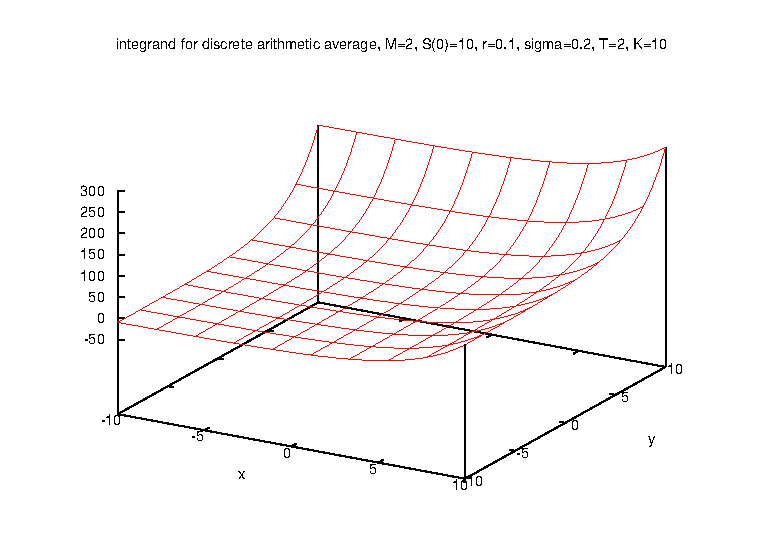
\includegraphics{task5_2}\\

\section*{Task 6}
See task6.cpp for code.

\section*{Task 7}
See task7.cpp for code. Below is a plot of the first 100 members of the Halton sequence for $d=2$ and 100 uniform random numbers on $(0,1)^2$. As we can see, the Halton sequence covers the unit square more evenly than uniformly distributed points, i.e. "gaps" between the points are not as big.
\\
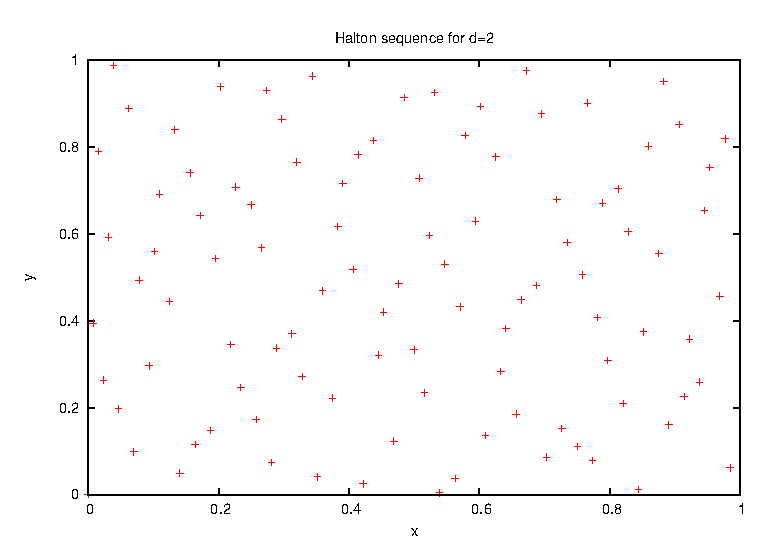
\includegraphics{task7_halton.eps}\\
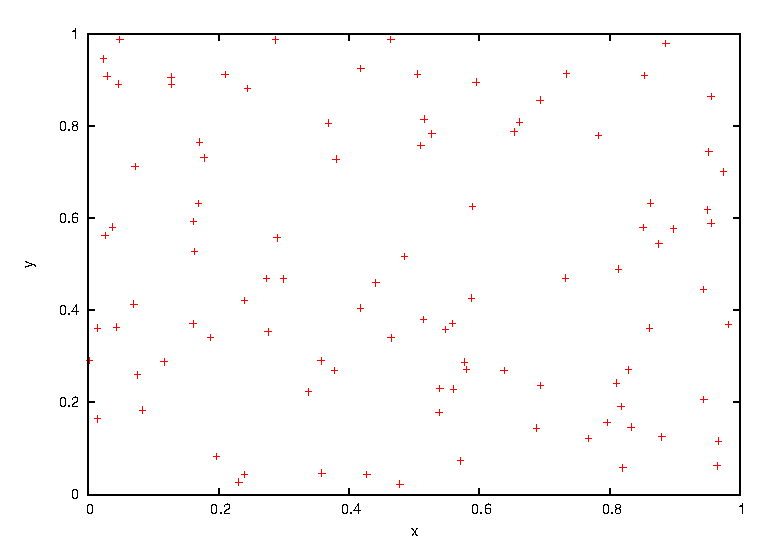
\includegraphics{task7_uniform.eps}\\

\section*{Task 8}
See task8.cpp for code.

\section*{Task 9}
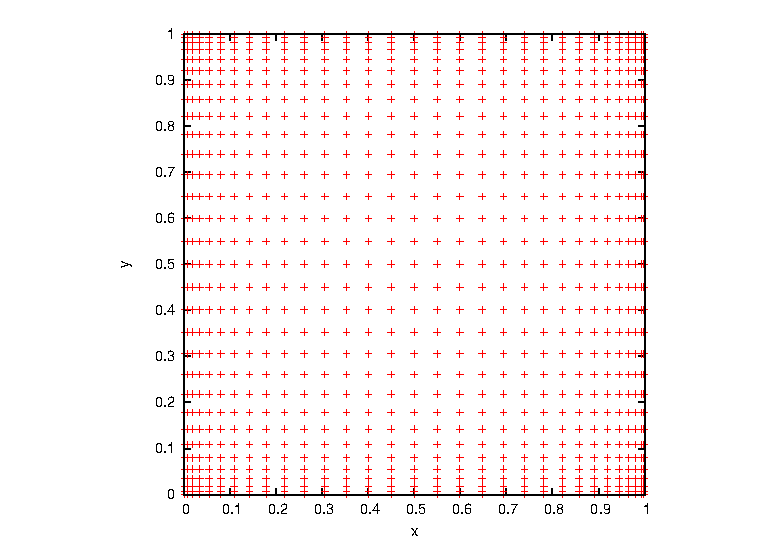
\includegraphics{task9_gauss}\\
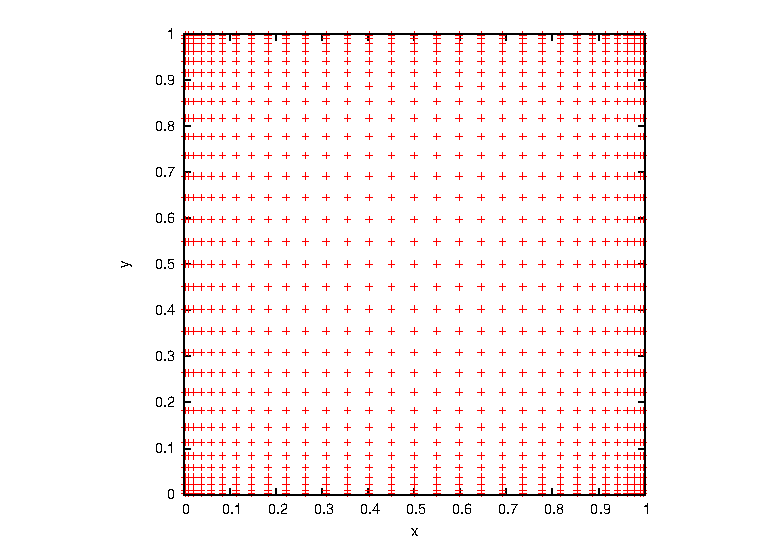
\includegraphics{task9_cc}\\
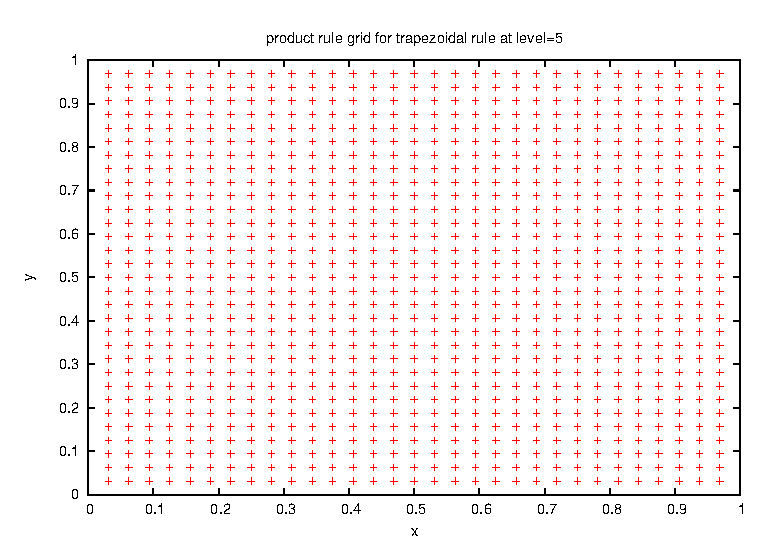
\includegraphics{task9_trapezoidal}\\

\section*{Task 10}
See task10.cpp for code.

\section*{Task 11}
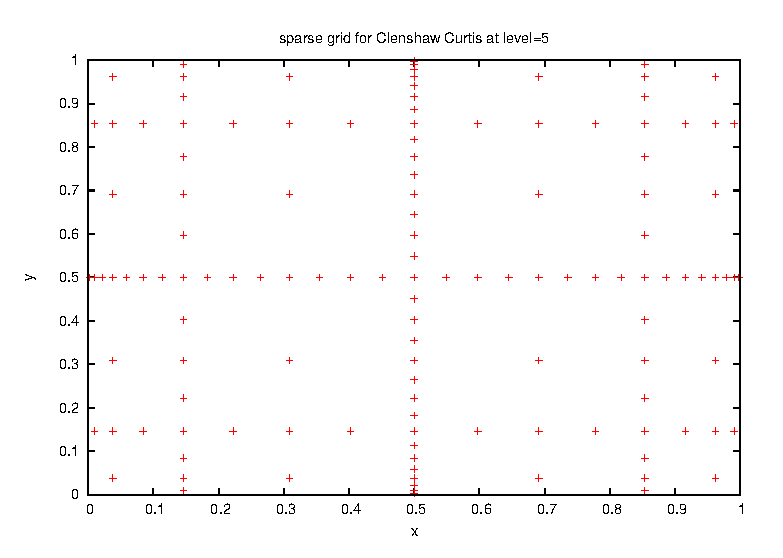
\includegraphics{task11_cc5}\\
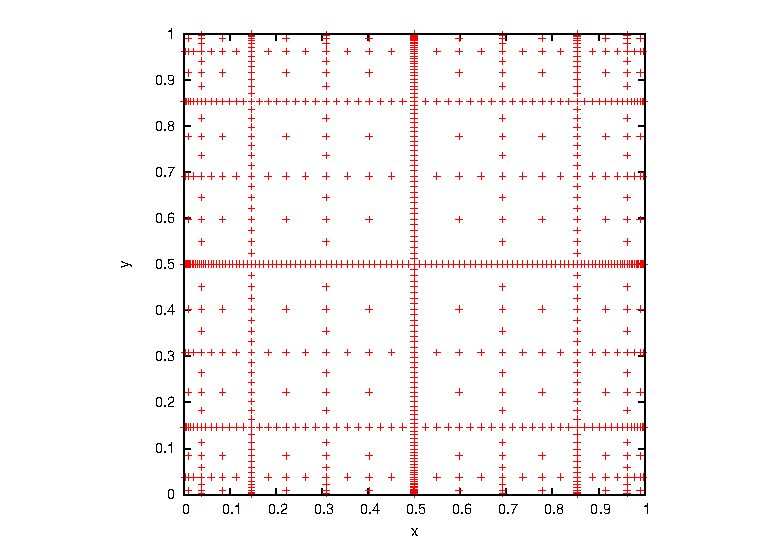
\includegraphics{task11_cc7}\\
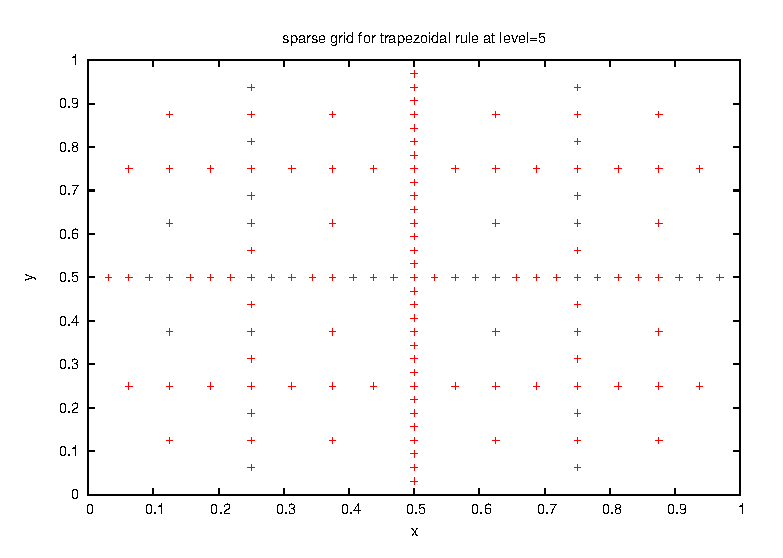
\includegraphics{task11_trap_5}\\
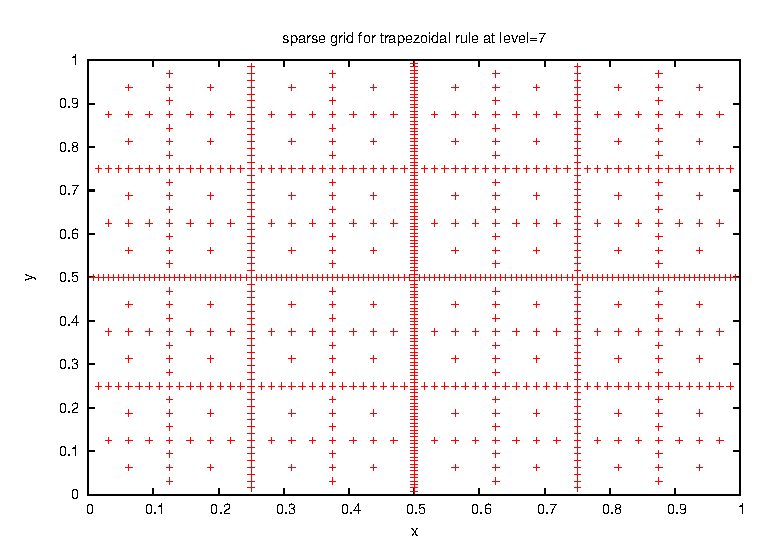
\includegraphics{task11_trap_7}\\

\section*{Task 12}
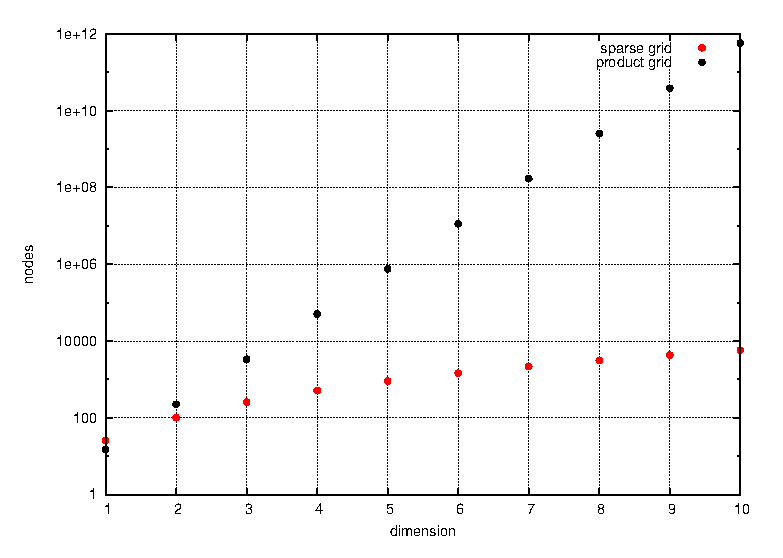
\includegraphics{task12}\\

\section*{Task 13}
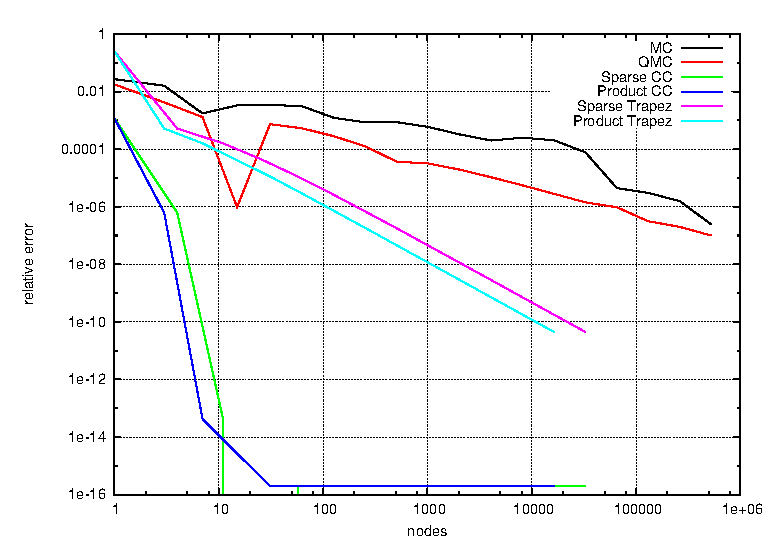
\includegraphics{task13_d1}\\
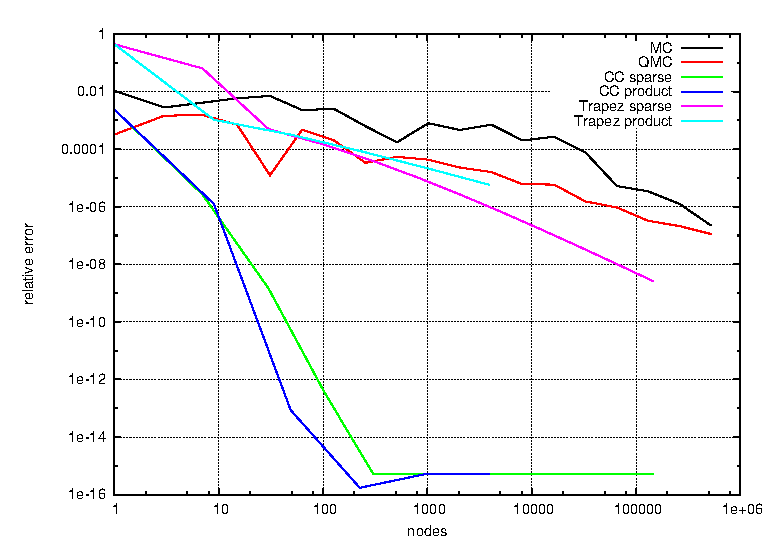
\includegraphics{task13_d2}\\
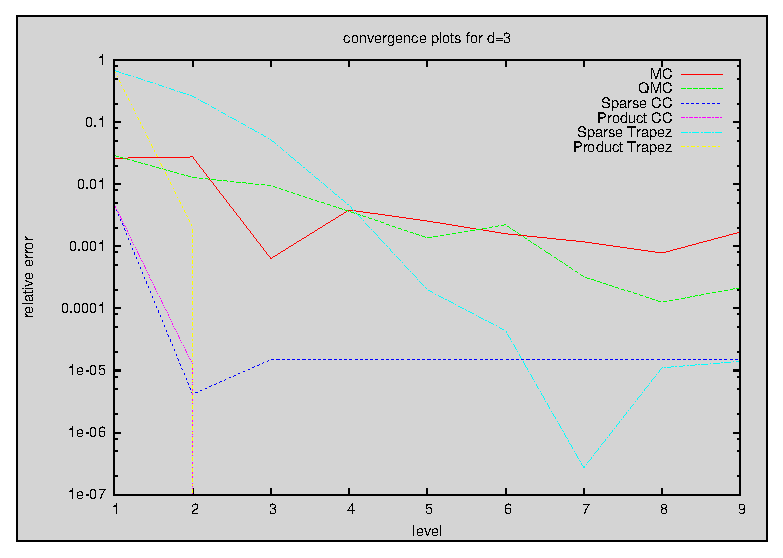
\includegraphics{task13_d4}\\
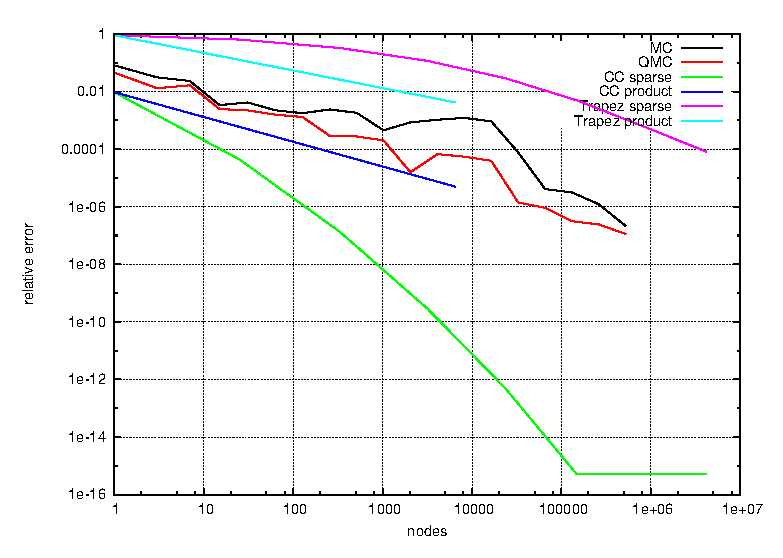
\includegraphics{task13_d8}\\

\section*{Task 14}
See task14.cpp/task15.cpp

\section*{Task 15}
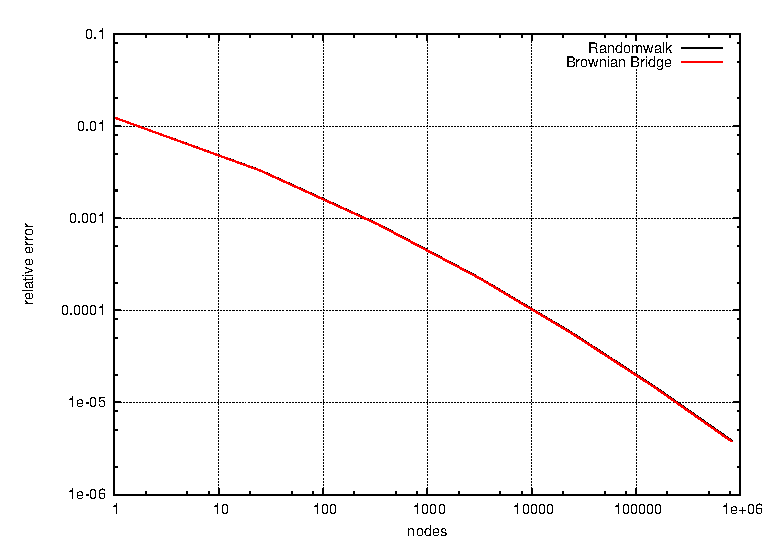
\includegraphics{task15}\\

\section*{Task 16}
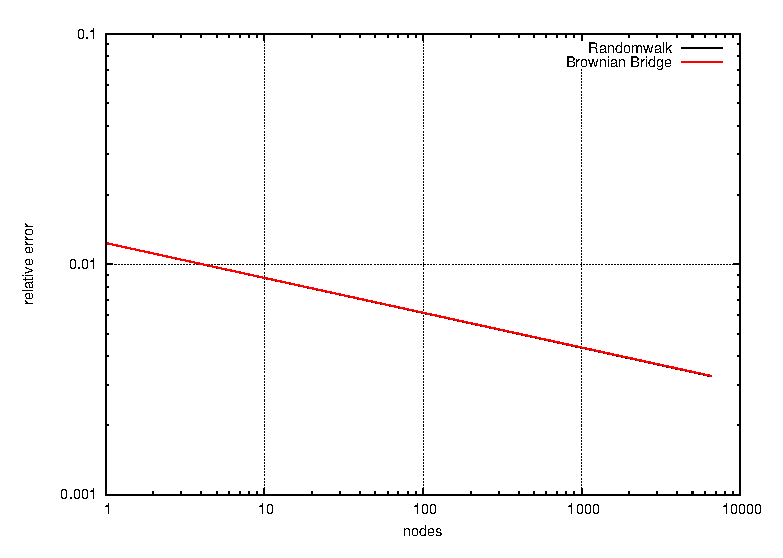
\includegraphics{task16_ccprod}\\
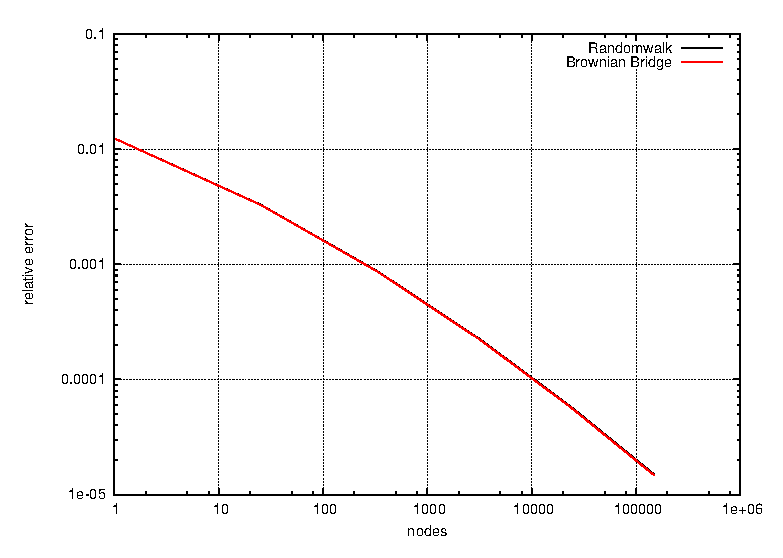
\includegraphics{task16_ccsparse}\\
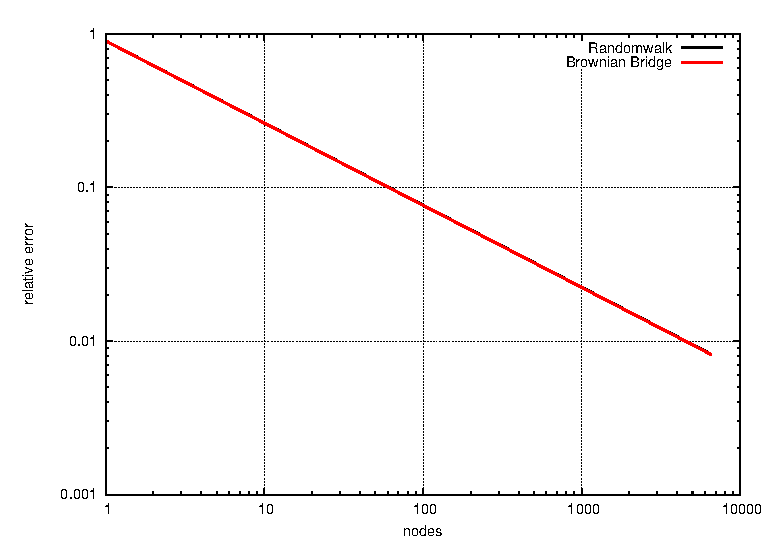
\includegraphics{task16_trapprod}\\
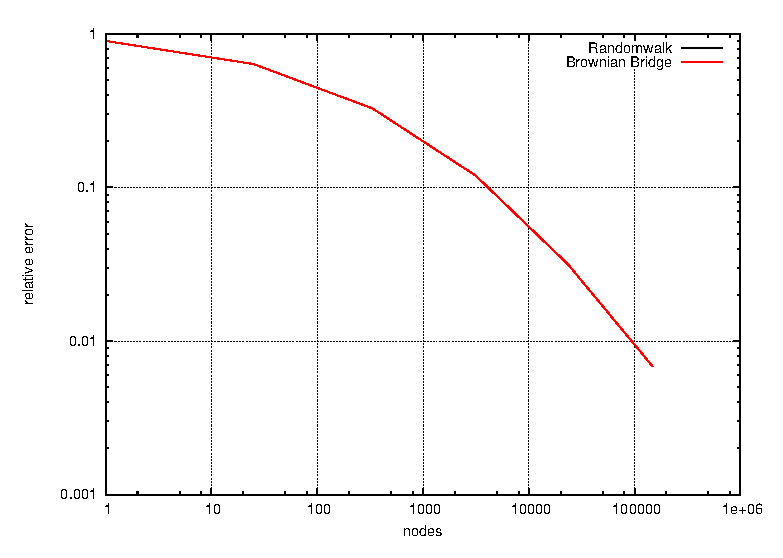
\includegraphics{task16_trapsparse}\\
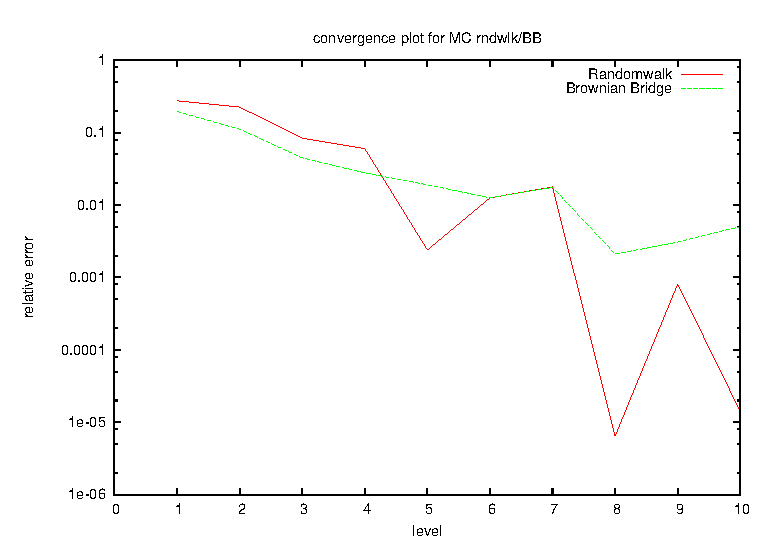
\includegraphics{task16_mc}\\
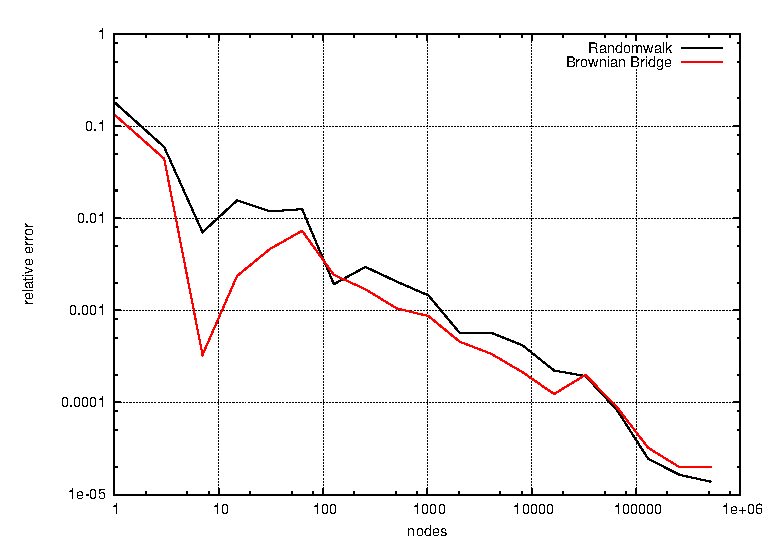
\includegraphics{task16_qmc}\\

\section*{Task 17}
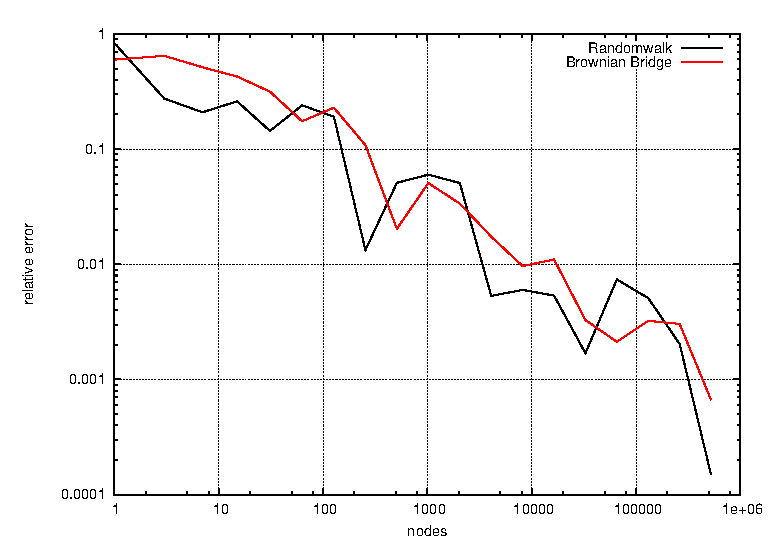
\includegraphics{task17_mc}\\
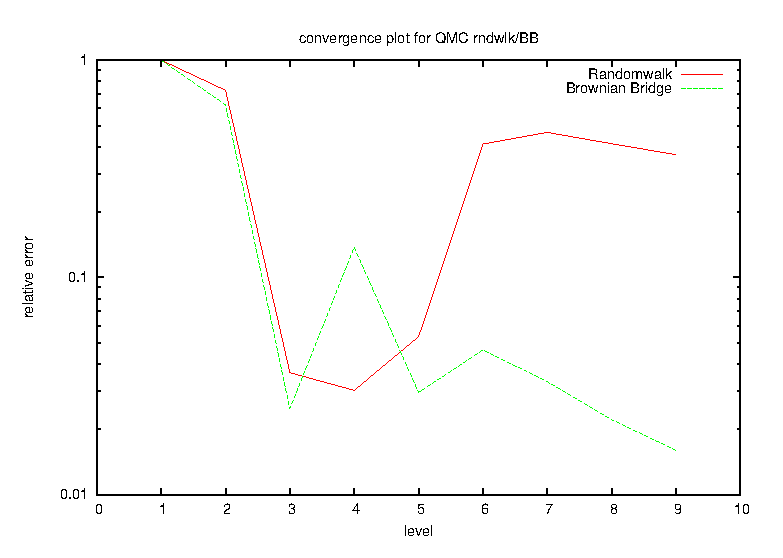
\includegraphics{task17_qmc}\\

\section*{Task 18}
It is almost always better to not use (Q)MC, since the other quadrature rules converge faster (even using full grids). Clenshaw-Curtis converges slightly faster than the Trapezoidal rule. In almost all cases sparse grids are preferrable Since they only give us a slightly worse convergences, but way less points of evaluation (see Task 12). But if everything else fails, (Q)MC works (but might converge slowly).
\end{document}
